% Rendimiento computacional unificado de los 4 casos
\subsection{Rendimiento Computacional}
\begin{frame}{Rendimiento computacional — Comparativa de los 4 casos}
    \vspace{0.1cm}
    \begin{columns}
        \begin{column}{0.5\textwidth}
            \centering
            {\footnotesize Caso 01: Problema de Hill}\\
            \vspace{0.1cm}
            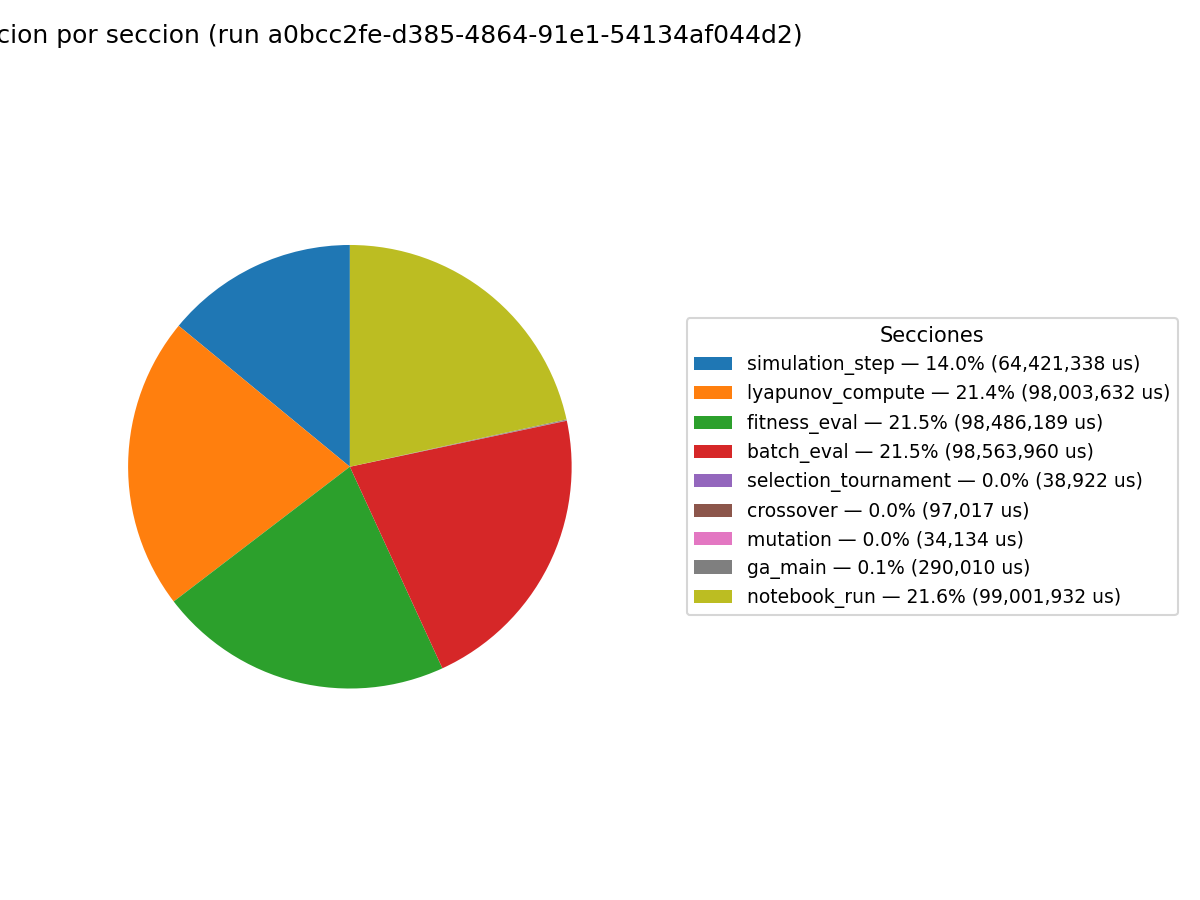
\includegraphics[width=\textwidth, height=0.3\textheight, keepaspectratio]{img/resultados/caso01-metricasTiempo.png}

            \vspace{0.25cm}
            {\footnotesize Caso 02: Problema de Sitnikov}\\
            \vspace{0.1cm}
            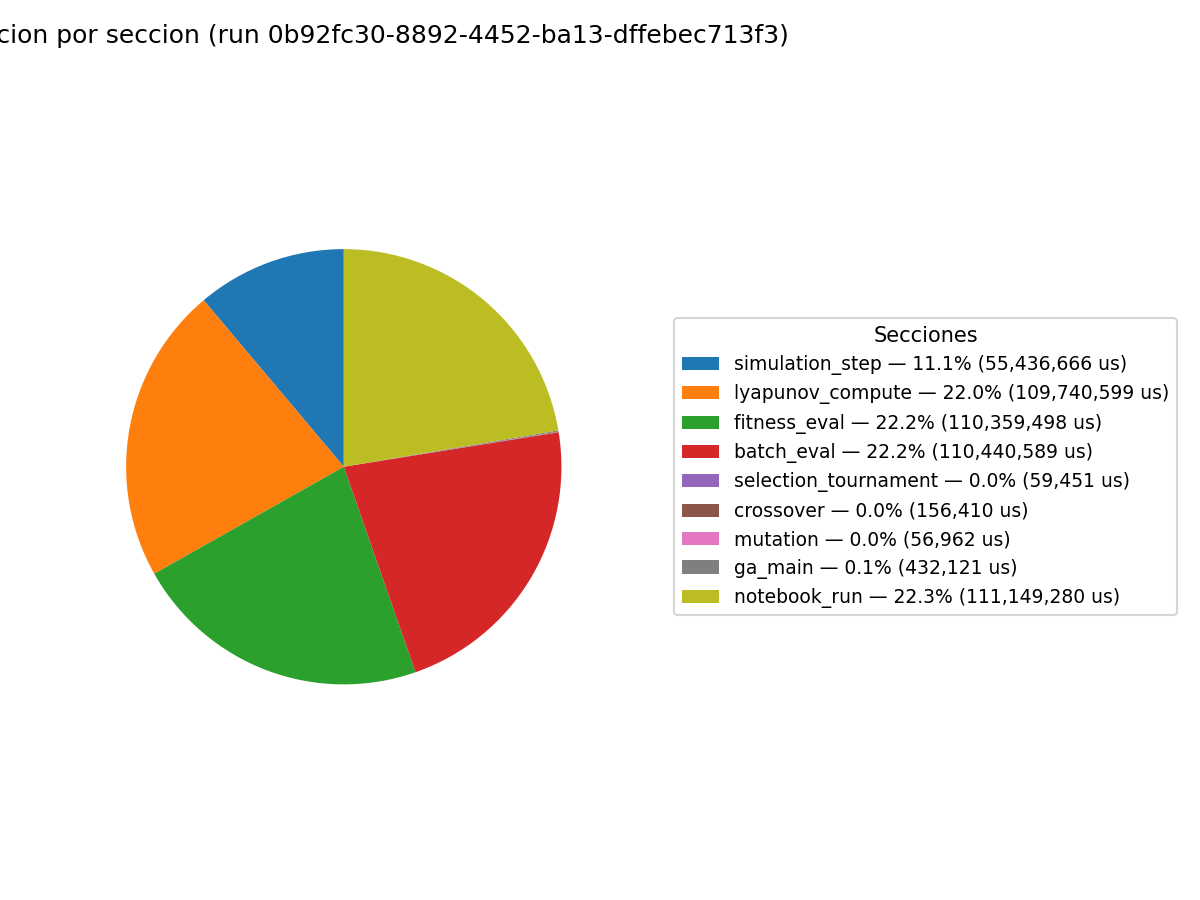
\includegraphics[width=\textwidth, height=0.3\textheight, keepaspectratio]{img/resultados/caso02-metricasTiempo.png}
        \end{column}
        \begin{column}{0.5\textwidth}
            \centering
            {\footnotesize Caso 03: Kepler pateado}\\
            \vspace{0.1cm}
            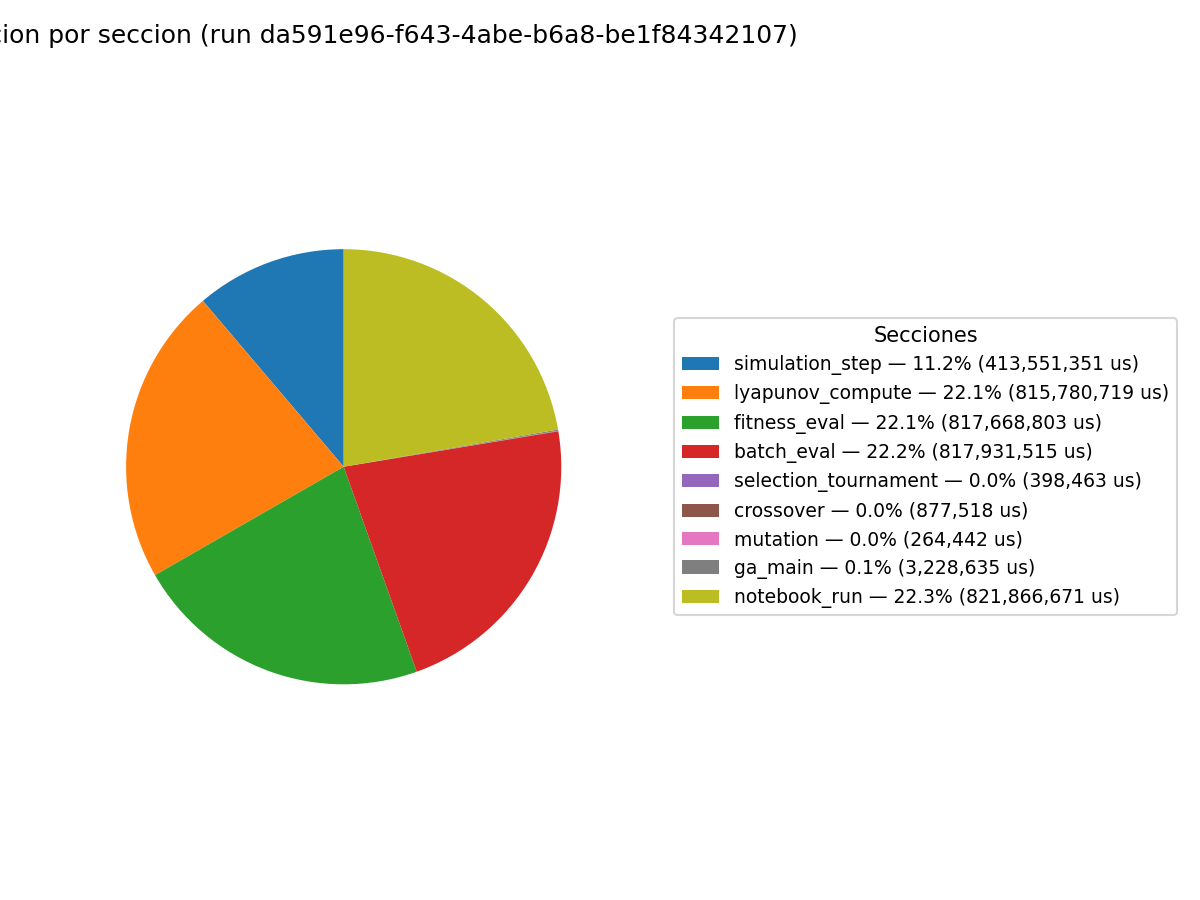
\includegraphics[width=\textwidth, height=0.3\textheight, keepaspectratio]{img/resultados/caso03-metricasTiempo.png}

            \vspace{0.25cm}
            {\footnotesize Caso 04: Sistema binario con intruso}\\
            \vspace{0.1cm}
            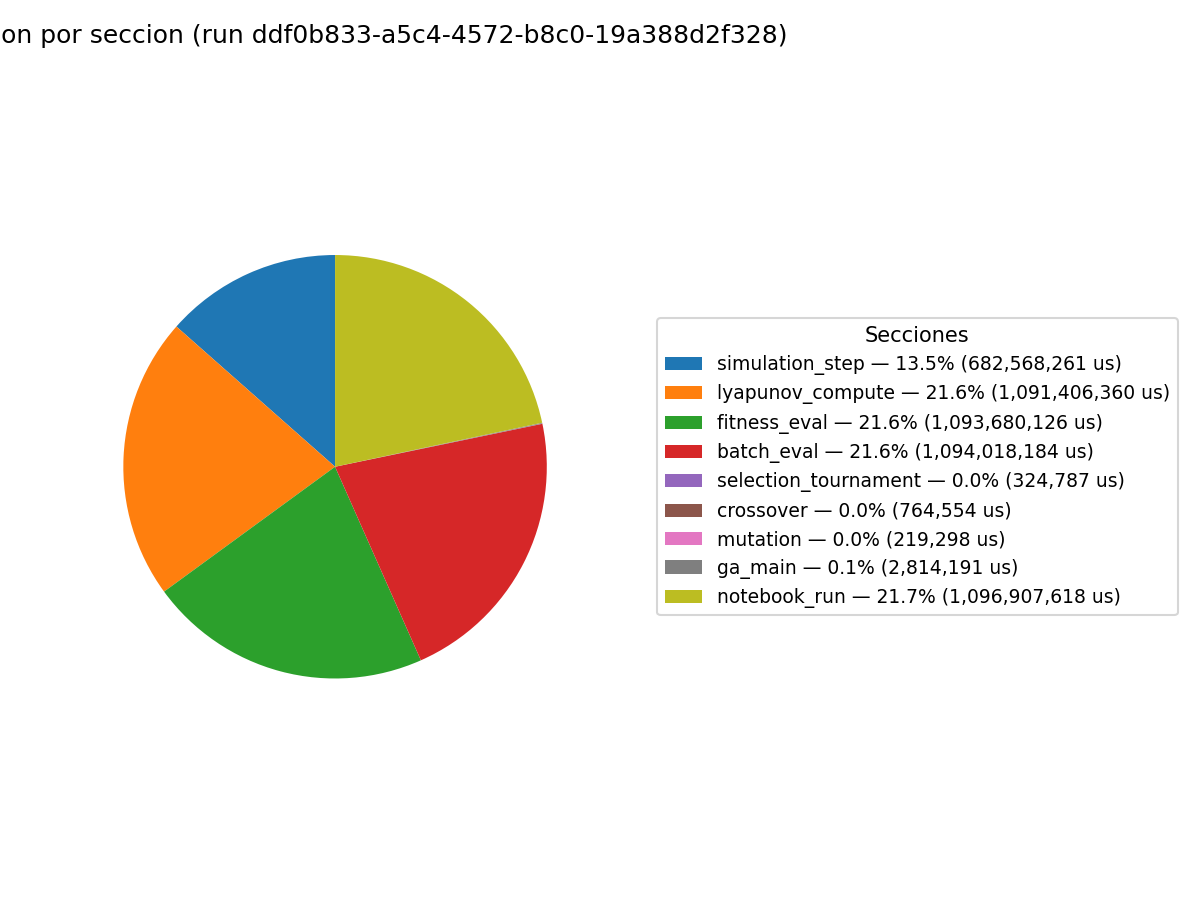
\includegraphics[width=\textwidth, height=0.3\textheight, keepaspectratio]{img/resultados/caso04-metricasTiempo.png}
        \end{column}
    \end{columns}
    \vspace{0.1cm}
    {\small Análisis comparativo de tiempos de ejecución para los 4 casos de prueba.~\textit{Autoría Propia}}
\end{frame}
